% From the repository root: latexmk -cd -pdf presentation/recommender-systems.tex
% Part 3, Track A. MMR code and reported results: origin/part3-mmr at 4a252ea.
% Recreate the figure PDFs with the two Python scripts in figures/.
\documentclass[aspectratio=169,9pt,t]{beamer}

\usepackage[T1]{fontenc}
\usepackage{lmodern}
\usepackage{booktabs}
\usepackage{tabularx}
\usepackage{tikz}
\usetikzlibrary{matrix}
\graphicspath{{figures/}{presentation/figures/}}

% Palette
\definecolor{Paper}{HTML}{F7F9F7}
\definecolor{Ink}{HTML}{142923}
\definecolor{Muted}{HTML}{47615A}
\definecolor{Accent}{HTML}{00775D}
\definecolor{Mint}{HTML}{A6F2D6}

\title[Movie recommendation]{MMR re-ranking on MovieLens 1M}
\subtitle{Track A \textperiodcentered{} Diversity and popularity bias}
\author{Mathis Fournier, David Ramos and Paul Lorenz}
\institute{Recommender Systems\\[0.10cm]Tampere University}
\date{} % Add a presentation date here if needed.

\newlength{\slidemargin}
\setlength{\slidemargin}{0.7cm}
\setbeamersize{text margin left=\slidemargin,text margin right=\slidemargin}
\setbeamercolor{normal text}{fg=Ink,bg=Paper}
\setbeamercolor{structure}{fg=Accent}
\setbeamercolor{alerted text}{fg=Accent}
\setbeamercolor{frametitle}{fg=Ink}
\setbeamercolor{footline}{fg=Muted}
\setbeamerfont{frametitle}{size=\LARGE,series=\bfseries}
\setbeamerfont{footline}{size=\scriptsize}
\setbeamertemplate{navigation symbols}{}
\setbeamertemplate{frametitle}{%
  \vspace{0.25cm}%
  \noindent\insertframetitle\par
  \vskip0.10cm
  {\color{Accent}\hrule width 0.65cm height 0.7pt}
  \vskip0.12cm
}
\setbeamertemplate{footline}{%
  \begin{beamercolorbox}[wd=\paperwidth,ht=2ex,dp=1.5ex,
    leftskip=\slidemargin,rightskip=\slidemargin]{footline}
    Team 14\enspace\textperiodcentered\enspace\insertsectionhead\hfill\insertframenumber
  \end{beamercolorbox}%
}

\begin{document}

% Cover
{
\setbeamercolor{background canvas}{bg=Ink}
\begin{frame}[plain,s,noframenumbering]
  \color{Paper}
  \vfill
  \begin{columns}[onlytextwidth,c]
    \begin{column}{0.71\textwidth}
      {\color{Mint}\rule{1.1cm}{1.5pt}\par}
      \vspace{0.23cm}
      {\bfseries\fontsize{21}{24}\selectfont\inserttitle\par}
      \vspace{0.22cm}
      {\large\insertsubtitle\par}
      \vspace{0.42cm}
      {\small\color{Mint}\insertauthor\par}
      \vspace{0.10cm}
      {\small\insertinstitute\par\insertdate\par}
    \end{column}
    \begin{column}{0.26\textwidth}
      \centering
      % A stylized user-item ratings matrix.
      
\begin{tikzpicture}[x=0.58cm,y=0.58cm]
        \foreach \x in {0,...,4} {
          \foreach \y in {0,...,4} {
            \fill[Paper,opacity=0.12,rounded corners=2pt]
              (\x,\y) rectangle ++(0.82,0.82);
          }
        }
        \foreach \x/\y in {0/3,1/0,1/2,2/4,3/1,3/3,4/2} {
          \fill[Mint,rounded corners=2pt] (\x,\y) rectangle ++(0.82,0.82);
        }
      \end{tikzpicture}
    \end{column}
  \end{columns}
  \vfill
\end{frame}
}


\section{Method}
\begin{frame}{Baseline recommender: Bayesian Personalized Ranking (BPR)}
  % Lecture 2.1, slide 4. Three users, three movies and three illustrative factors.
  \begin{columns}[onlytextwidth,c]
    \begin{column}{0.56\textwidth}
      \centering
      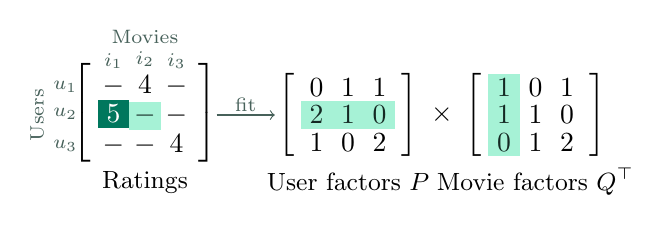
\begin{tikzpicture}[
        factors/.style={matrix of math nodes, ampersand replacement=\&,
          nodes={minimum width=0.40cm,minimum height=0.35cm,inner sep=0pt},
          inner sep=1pt,left delimiter={[},right delimiter={]}},
        picked/.style={fill=Mint,text=Ink},
        caption/.style={font=\small}, axis/.style={font=\scriptsize,text=Muted,inner sep=1pt}
      ]
        \matrix (R) [factors] at (0,0) {
          - \& 4 \& - \\
          |[fill=Accent,text=white]| 5 \& |[picked]| - \& - \\
          - \& - \& 4 \\
        };
        \foreach \n in {1,2,3} {
          \node[axis,anchor=south] at (R-1-\n.north) {$i_{\n}$};
          \node[axis,anchor=east,xshift=-6pt] at (R-\n-1.west) {$u_{\n}$};
        }
        \node[axis] at (0,0.99) {Movies};
        \node[axis,rotate=90] at (-1.37,0) {Users};
        \node[caption] at (0,-0.85) {Ratings};

        \draw[->,Muted] (0.91,0) -- (1.65,0) node[midway,above,axis] {fit};
        \matrix (P) [factors,row 2/.style={nodes=picked}] at (2.58,0) {
          0 \& 1 \& 1 \\
          2 \& 1 \& 0 \\
          1 \& 0 \& 2 \\
        };
        \node at (3.77,0) {$\times$};
        \matrix (Q) [factors,column 1/.style={nodes=picked}] at (4.96,0) {
          1 \& 0 \& 1 \\
          1 \& 1 \& 0 \\
          0 \& 1 \& 2 \\
        };
        \node[caption] at (2.58,-0.85) {User factors $P$};
        \node[caption] at (4.96,-0.85) {Movie factors $Q^\top$};
      \end{tikzpicture}
    \end{column}
    \begin{column}{0.42\textwidth}
      \textbf{Movie score}\quad $s_{ui}=\mathbf p_u^\top\mathbf q_i+b_i$\par\smallskip
      For $u_2$, BPR maximizes the probability that the 5-star movie $i_1$
      outranks the unrated $i_2$.\par\smallskip
      $\Pr(i_1\succ i_2\mid u_2)=\sigma(s_{21}-s_{22})$
    \end{column}
  \end{columns}

  \vfill
  \textbf{Training loss}\quad
  $\displaystyle \min_{\Theta}\;\sum_{\text{examples}}\ell+\lambda\lVert\Theta\rVert^2$
  \hfill{\small\color{Muted}Lecture 2.1, slides 4 and 12}\par\medskip
  \begin{columns}[onlytextwidth,T]
    \begin{column}{0.28\textwidth}
      \textbf{Pointwise}\par\smallskip
      $\ell=(r_{ui}-s_{ui})^2$\par\smallskip
      Fit one observed rating $r_{ui}$.
    \end{column}
    \begin{column}{0.36\textwidth}
      \alert{\textbf{Pairwise (BPR, selected)}}\par\smallskip
      $\ell=-\log\sigma(s_{ui}-s_{uj})$\par\smallskip
      Pair a 4--5 star $i$ with an unrated $j$.
    \end{column}
    \begin{column}{0.31\textwidth}
      \textbf{Listwise (example)}\par\smallskip
      $\ell=1-\mathrm{NDCG@10}(\pi_u)$\par\smallskip
      Score the ranked list $\pi_u$.
    \end{column}
  \end{columns}

  \vfill
  \textbf{Test results}\hfill{\small\color{Muted}777 users, mean $\pm$ 95\% CI across five seeds}\par\smallskip
  \begin{tabular*}{\linewidth}{@{\extracolsep{\fill}}lrrrr@{}}
    \toprule
    Model & Precision@10 & Recall@10 & NDCG@10 & Catalogue coverage \\
    \midrule
    BPR-MF & $0.1863\pm0.0018$ & $0.0746\pm0.0018$ & $0.2098\pm0.0012$ & $0.1947\pm0.0029$ \\
    \bottomrule
  \end{tabular*}
\end{frame}

% Worked example from the seed-0 BPR fit, MovieLens user 1186.
\begin{frame}{Maximal Marginal Relevance (MMR)}
  \setlength{\belowdisplayskip}{3pt}
  \setlength{\belowdisplayshortskip}{3pt}
  To balance relevance and genre variety, pick the remaining movie that maximizes
  \hfill{\small\color{Muted}Lecture 5.1, slide 9}
  \[
    \lambda \times \text{scaled BPR score}
    \;-\; (1-\lambda) \times \text{highest genre similarity to a movie already picked}
  \]

  \textbf{Our implementation}\par\smallskip
  Take BPR's top 100 unrated movies per user and scale their scores to $[0,1]$.
  The distance between two movies is \alert{\textbf{one minus the cosine similarity}}
  of their 18-dimensional binary genre vectors.
  Keep BPR's first pick and use MMR for the next nine.
  \par\smallskip
  We swept $\lambda$ from 1 to 0 in steps of 0.05 and chose \alert{\textbf{0.55}},
  the smallest value retaining at least 95\% of BPR's validation NDCG@10.

  \bigskip
  \textbf{Example:} User 1186, $\lambda=0.55$ \par\smallskip
  \renewcommand{\arraystretch}{1.12}
  \begin{tabularx}{\linewidth}{@{}Xlrr@{}}
    \toprule
    \textbf{Film} & \textbf{MovieLens genres} & \textbf{BPR rank} & \textbf{MMR rank} \\
    \midrule
    Halloween (1978)          & Horror         & 1 & 1 \\
    Dracula (1931)            & Horror         & 2 & Outside top 10 \\
    Back to the Future (1985) & Comedy, Sci-Fi & 3 & \alert{\textbf{2}} \\
    \bottomrule
  \end{tabularx}

  \smallskip
  MMR dropped the second horror film, \textit{Dracula}, which the user later rated four stars.
\end{frame}

\section{Results and trade-offs}
\begin{frame}{Accuracy and intra-list diversity}
  \begin{columns}[onlytextwidth,T]
    \begin{column}{0.59\textwidth}
      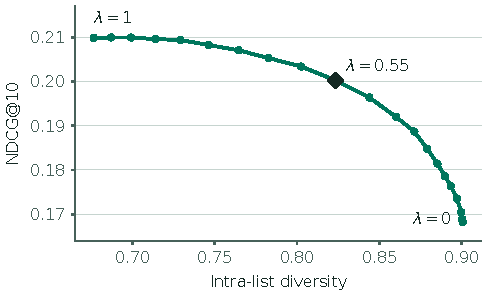
\includegraphics[width=\linewidth]{frontier.pdf}
    \end{column}
    \begin{column}{0.38\textwidth}
      With $\lambda=1$ we get the original BPR list. Lowering it to 0.80 increased
      mean genre distance from 0.677 to 0.729. NDCG@10 changed by less than 0.001.

      \medskip
      Below our chosen setting of 0.55, we lost accuracy more quickly.
      Going from 0.55 to 0 increased genre distance by another 0.077,
      while NDCG@10 fell from 0.2002 to 0.1682.
    \end{column}
  \end{columns}
  \medskip
  {\small\color{Muted}Each dot is one of 21 settings, averaged over 777 test users
  and five BPR fits. Genre distance averages all 45 pairs in a top ten.
  NDCG@10 rewards placing films the user later rated highly near the top.}
\end{frame}

\begin{frame}{Catalogue exposure and genre calibration}
  \begin{columns}[onlytextwidth,c]
    \begin{column}{0.56\textwidth}
      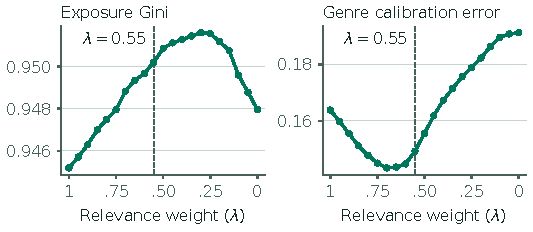
\includegraphics[width=\linewidth]{exposure-calibration.pdf}
    \end{column}
    \begin{column}{0.41\textwidth}
      \small
      \renewcommand{\arraystretch}{1.26}
      \begin{tabularx}{\linewidth}{@{}Xrr@{}}
        \toprule
        \textbf{Test metric} & \textbf{BPR} & \textbf{$\lambda=0.55$} \\
        \midrule
        Intra-list diversity & 0.677 & 0.823 \\
        Catalogue coverage & 19.47\% & 18.46\% \\
        Exposure Gini & 0.945 & 0.950 \\
        Calibration error & 0.164 & 0.149 \\
        \bottomrule
      \end{tabularx}
    \end{column}
  \end{columns}
  \medskip
  At 0.55, the genre mix was closer on average to what each user had liked before.
  Lowering $\lambda$ further made that fit worse. We also recommended fewer distinct
  movies than BPR did, and a larger share of recommendations went to the same titles.

  \smallskip
  {\small\color{Muted}Gini counts appearances across all 3,706 films, including zeroes.
  Calibration compares each list's genre mix with the user's previous likes (4--5 stars) using base-2
  Jensen--Shannon divergence. Two users had no previous likes, leaving 775 for calibration.}
\end{frame}

\section{Cost and interpretation}
\begin{frame}{Cost of the selected setting}
  At $\lambda=0.55$, MMR retained 95.04\% of BPR's validation NDCG@10.
  For each of the 777 test users, we averaged the change in NDCG@10 from BPR to MMR
  across five fits.

  \medskip
  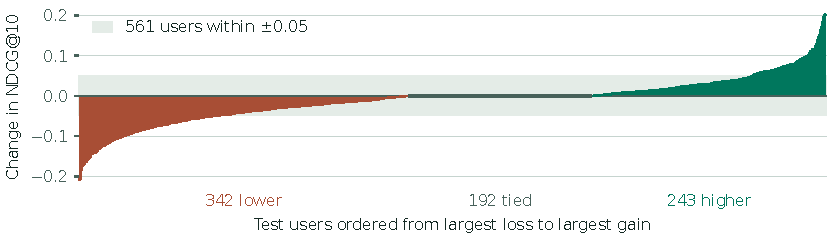
\includegraphics[width=\linewidth]{ranked-cost.pdf}

  \medskip
  Mean test NDCG@10 fell by 4.6\%. All 777 users received more genre variety
  on average across the five fits.

  \smallskip
  {\small\color{Muted}Paired mean NDCG@10 change $-0.0096$ (95\% user-bootstrap interval
  $-0.0135$ to $-0.0059$). Mean genre distance rose by $0.1468$ ($0.1417$ to $0.1521$).}
\end{frame}

\section{One number we cannot explain}
\begin{frame}{One number we cannot explain}
  At $\lambda=0.55$, all 777 users gained genre variety on average. Yet catalogue coverage
  fell from 19.47\% to 18.46\%, or about \alert{\textbf{38 fewer distinct films}} per fit.

  \medskip
  \textbf{Some films appeared in far more top tens than we expected}\hfill
  {\small\color{Muted}Rounded means across five fits}\par\smallskip
  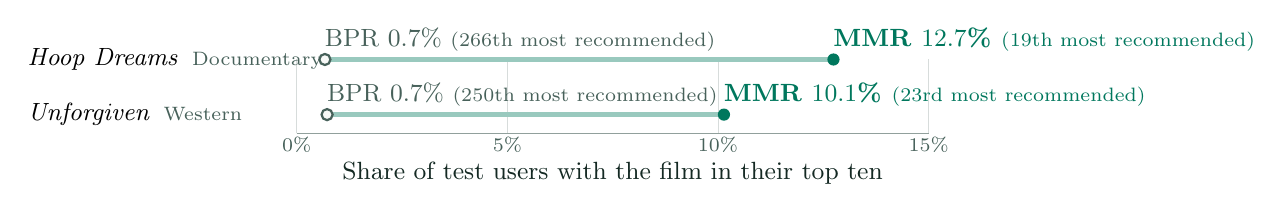
\begin{tikzpicture}[x=0.535cm,y=0.70cm,font=\small,
    point label/.style={anchor=south west,yshift=3pt,inner sep=0pt,outer sep=0pt}]
    \foreach \x in {0,5,10,15} {
      \draw[Muted!22,line width=0.35pt] (\x,-0.34) -- (\x,1);
      \node[below=1pt,inner sep=0pt,font=\scriptsize,text=Muted] at (\x,-0.34) {\x\%};
    }
    \draw[Muted!60,line width=0.4pt] (0,-0.34) -- (15,-0.34);
    \node[anchor=north,inner sep=0pt,font=\small,text=Ink] at (7.5,-0.85)
      {Share of test users with the film in their top ten};
    % Counts are means across five fits, each with the same 777 users.
    % Ranks use unrounded top-ten appearances across fits; ties share a rank.
    \foreach \film/\genre/\row/\bprcount/\mmrcount/\bprrank/\mmrrank in {
      Hoop Dreams/Documentary/1/5.2/99/266th/19th,
      Unforgiven/Western/0/5.6/78.8/250th/23rd} {
      \pgfmathsetmacro{\bpr}{100*\bprcount/777}
      \pgfmathsetmacro{\mmr}{100*\mmrcount/777}
      \node[anchor=west,inner sep=0pt] at (-6.4,\row)
        {\textit{\film}\enspace{\scriptsize\color{Muted}\genre}};
      \draw[Accent!40,line width=2pt] (\bpr,\row) -- (\mmr,\row);
      \draw[Muted,fill=Paper,line width=0.8pt] (\bpr,\row) circle[radius=2pt]
        node[point label,text=Muted]{BPR \pgfmathprintnumber[fixed,precision=1]{\bpr}\%
          {\scriptsize(\bprrank\ most recommended)}};
      \fill[Accent] (\mmr,\row) circle[radius=2.2pt]
        node[point label,text=Accent,font=\small\bfseries]{MMR \pgfmathprintnumber[fixed,precision=1]{\mmr}\%
          {\scriptsize\mdseries(\mmrrank\ most recommended)}};
    }
  \end{tikzpicture}\par
  \bigskip
  \textbf{How we could investigate}\par\smallskip
  \textbf{1. Would random swaps also cost 38 films?} For each user, replace as many picks as
  MMR did, sampling from similar BPR ranks in their top 100. Repeat and compare coverage.\par\smallskip
  \textbf{2. Could another film give the same variety?} Where MMR added \textit{Hoop Dreams},
  try a different candidate with identical genre tags and a similar BPR score. Measure how much
  coverage changes with genre diversity held fixed.
\end{frame}

\section{References}
\begin{frame}{References}
  \textbf{Course slides}\par\smallskip
  Kostas Stefanidis. \textit{Recommender Systems}, Tampere University.\par
  Lecture 2.1, \textit{Matrix Factorization}, slides 4 and 12.\par
  Lecture 3.1, \textit{Evaluation}, slides 7--8.\par
  Lecture 5.1, \textit{Diversity, Novelty and Popularity Bias}, slides 8--9.

  \bigskip
  \textbf{BPR}\par\smallskip
  Aleksandr Milogradskii, Oleg Lashinin, Alexander P, Marina Ananyeva and Sergey Kolesnikov (2024).
  \textit{Revisiting BPR: A Replicability Study of a Common Recommender System Baseline.}
  ACM RecSys. \href{https://arxiv.org/pdf/2409.14217}{\color{Accent}arXiv:2409.14217}

  \bigskip
  \textbf{Maximal Marginal Relevance}\par\smallskip
  Julian McAuley (2022). \textit{Personalized Machine Learning}. Cambridge University Press.\par
  \href{https://cseweb.ucsd.edu/~jmcauley/pml/pml_book.pdf}{\color{Accent}Section 10.3.1}
  gives the MMR rule. Section 10.4 shows how the top ten changes with $\lambda$.
  \href{https://cseweb.ucsd.edu/~jmcauley/pml/code/chap10.html}{\color{Accent}Worked example and code.}\par\smallskip
  {\small \href{https://doi.org/10.1145/290941.291025}{\color{Accent}Carbonell and Goldstein}
  introduced MMR at SIGIR in 1998.}
\end{frame}

\end{document}
